\section{واحد مدیریت ترمیم و الگوریتم‌ها}

\subsection*{دو تراکنش زیر چه قوانینی را تقض کرده‌اند؟ توضیح دهید}

\begin{LTR}
    \begin{table}[h]
        \begin{RTL}
        \end{RTL}
        \centering
            \begin{tabular}{c|c}
                $T_1$ & $T_2$ \\ \hline
                : & : \\
                : & : \\
                : & : \\
                : & : \\
                Failure & : \\
                : & Commit \\
                : & Failure
            \end{tabular}
    \end{table}
\end{LTR}

در تراکنش $T_1$ قانون Atomicity رعایت نشده است، چرا که حین اجرا به مشکل بر خورده
و تراکنش اول به پایان نرسیده است. یکی از مهم‌ترین قوانین ACID بخش Atomicity است
که تراکنش یا باید کامل انجام شود که کامیت شود یا نهایتا سقوط کند.

در تراکنش $T_2$ قانون Duribility رعایت نشده است. یعنی تراکنش به صورت کامل انجام
شده است و حتی کامیت هم صورت گرفته اما در حافظه و یا قسمتی که مربوط به ثبت داده
این تراکنش است منعکس نشده است.

\subsection{انواع خطا‌های مربوط به سیستم دیتابیس}

\subsubsection{خطا‌های تراکنشی}

\begin{enumerate}
    \item خطای منطقی: تراکنش با توجه به قوانینی که برای آن تعریف کردیم، اشتباه
    انجام شود، مانند خطای تقسیم بر صفر. این نوع خطا بر روی کل دیتابیس تاثیر گذار
    نیست
    \item خطای سیستمی: مانند Kill شدن تراکنش‌ها به هر دلیلی
\end{enumerate}

\subsubsection{خطا‌های سیستمی}

خطای سیستمی می‌تواند مربوط به سخت‌افزار و نرم‌افزار شود، برای مثال سیستم هنگ
کرده باشد، رم پر شده باشد یا از نظر سخت‌افزاری مشکلی برای آن پیش آمده باشد.

\subsubsection{خطای رسانه‌ای}

خرابی حافظه (دیسک) که می‌تواند سخت‌افزاری هم باشد اما بخش بسیار مهم یک سیستم
دیتابیسی را شامل می‌شود که می‌تواند روی همه داده‌ها تاثیر گذار باشد.

\subsubsection*{یادآوری}

واحد مدیریت همروندی مسئول برقرار خاصیت Isolation است در حالی که واحد مدیریت
ترمیم مسئول انجام شدن کامل تراکنش‌ها و خاصیت Duribility است.

\subsection{روال دسترسی به داده‌ها برای انجام تراکنش}

% @startuml
% package Storage {
%   package Buffer {
%     [AB] as "A"
%     [BB] as "B"
%   }
%   package TransactionsA {
%     [A1] as "A"
%     [B1] as "B"
%   }
%   package TransactionsB {
%     [An] as "An"
%   }
% }

% package Media {
%    database DB {
%     [A]
%     [B]
%   }
% }

% A --> Buffer: "Input()"
% Buffer --> B: "Output()"

% A1 --> Buffer: "Read()"
% B1 <-- Buffer: "Write()"
% @enduml

\begin{figure}
    \centering
    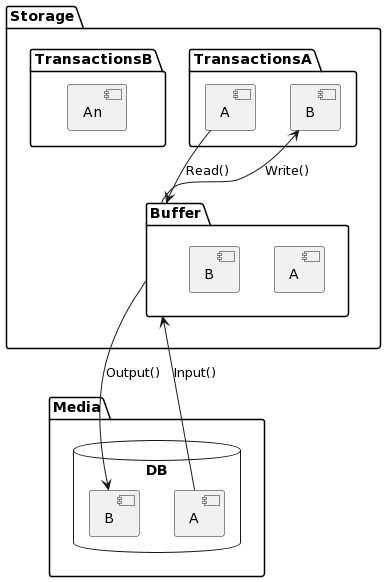
\includegraphics[width=0.3\textwidth]{umls/media.png}
    \caption{روال دسترسی به داده برای انجام تراکنش}
    \label{fig:media}
\end{figure}

داده‌های دیتابیس روی رسانه‌ها قرار دارند که به منظور پردازش آنها توسط
تراکنش‌ها،‌ باید به طور موقت به بخشی از حافظه اصلی منتقل شوند که آنرا بافر
\footnote{Buffer} می‌گوییم. آوردن داده از دیسک به بافر و بازگرداندن نتایج از
بافر به دیسک (معمولا به صورت بلاک‌های حافظه) توسط عملگر‌هایی (توابع) انجام
می‌شود که \lr{input()} و \lr{output()} نامیده می‌شود. هر تراکنشی که می‌خواهد با
داده‌ای کار کند، یک کپی از آن داده در بافر را در ناحیه کاری \footnote{Workarea}
خاص خود می‌برد و دسترسی‌های بعدی آن تراکنش روی کپی محلی اش انجام می‌شود و پس از
اتمام کار، این کپی محلی به بافر منقل می‌شود. باز هم برای این منظور نیاز به
عملگردهایی داریم که آنها را به ترتیب \lr{Read()} و \lr{Write()} می‌نامیم. شکل
\ref{fig:media} این موضوع را نشان می‌دهد. به طور خلاصه، خواندن و نوشتن روی
داده‌ها در workarea رخ می‌دهد که بعد از آن انتقال داده‌ها اول روی حافظه اصلی و
منطقی (بافر) صورت می‌گیرد و در نهایت از حافظه اصلی به حافظه جانبی و یا دیسک منقل
می‌شود.

\subsection*{نکته}

اگر داده در بافر حضور نداشته باشد درخواست خواندن را به دیسک ارسال می‌کند.

\subsection{الگوریتم‌های ترمیم}

الگوریتم‌های ترمیم برای حفظ جامیت و پایداری شامل دو مرحله می‌شوند، (به طور کلی
همان بک‌آپ و ری‌استور کردن داده‌ها می‌باشد)

\subsubsection{مرحله اول}

در این مرحله، حین اجرای تراکنش اطلاعاتی برای ترمیم نیاز است را در جایی ثبت
می‌کند.

\subsubsection{مرحله دوم}

در این مرحله، بعد از آنکه سیستم بالا آمد و وضعیت کلی مناسبی داشت اطلاعاتی که در
مرحله قبل ثبت شده در این مرحله خوانده می‌شود تا خواص Atomicity و Duribility
برقرار باشد.

\subsection*{طبق خاصیت Duribility}

اثرات تراکنشی که انجام شده باید دائمی و همیشگی باشد.

\subsection*{طبق خاصیت Atomicity}

تراکنشی که نیمه کاره متوقف شده است نباید هیچ اثری در دیتابیس داشته باشد.

\subsection{عملیات Redo}

زمانی عملیات را Redo می‌کنیم که تراکنش به صورت کامل کامیت شده و در انعکاس
اطلاعات در حافظه به مشکل خورده است (توجه شود تمام فرایند از اول انجام می‌شود).

\subsection{عملیات Undo}

زمانی عملیات را Undo می‌کنیم که خاصیت جامیعت نقض شده باشد. برای مثال تراکنش ساقط
شده باشد. به خاطر همین دستورات را مرحله به مرحله خنثی می‌کنیم (عملیات Undo از
پایین به بالا انجام می‌شود. از آخرین دستور تا اولین دستور).

\subsection{رویکرد‌های الگوریتم ترمیم}

\begin{itemize}
    \item کارنامه \footnote{\lr{Log based}}
    \item رونوشت \footnote{\lr{Shadow paging}}
\end{itemize}

\subsection{رویکرد کارنامه}

در این رویکرد اطلاعات برای حفظ ترمیم، در حافظه پایدار نوشته می‌شود. هر دستور
تراکنش رکوردی به نام رکورد کارنامه به شکل ساختار زیر می‌نویسد:

\begin{itemize}
    \item در ابتدا برای شروع تراکنش $T_i$ رکورد $<T_i, start>$ نوشته می‌شود
    \item دستور نوشتن بر روی منبع $X$ از تراکنش $T_i$ به صورت $<T_i, X, V_1,
    V_2>$ می‌نویسم. به معنای آن است که تراکنش مورد نظر بر روی منبع $X$ مقدار
    $V_2$ که مقداری جدید است را جایگذین مقدار $V_1$ کرده است.
    \item بعد از اجرای کامل دستورات تراکنش رکورد $<T_i, commit>$ را می‌نویسد.
\end{itemize}

\subsubsection*{نکته}

در این رویکرد حافظه بافر (حافظه ناپایدار) وجود ندارد و شایع‌ترین روش انجام
ترمیم، رویکرد کارنامه می‌باشد که انعکاس تغییرات را روی دیتابیس به سه شکل زیر
انجام می‌دهد:

\begin{itemize}
    \item انعکاس معوق تغییرات در دیتابیس \footnote{\lr{Deferred Database
    Modification}}
    \item انعکاس فوری تغییرات در دیتابیس \footnote{\lr{Immediate Database
    Modification}}
    \item روش نقاط بازرسی \footnote{\lr{Checkpoints}} (معمولا کارایی بهتری را
    ارائه می‌هد)
\end{itemize}

\subsubsection{\lr{Partial Commit}}

اجرای آخرین دستور تراکنش

\subsection{انعکاس معوق تغییرات در دیتابیس}

در این روش، رکورد‌های انجام تغییرات در کارنامه ثبت می‌شوند اما اعمال نهایی
(انعکاس) این تغییرات روی رسانه (یعنی اجرای واقعی write ها در دیتابیس) بعد از
اجرای آخرین دستور تراکنش یعنی \lr{Partial commit} به تعویق می‌افتد.

وقتی در تراکنش‌ها نوشتنی صورت می‌گیرد، این دستور در دیتابیس اعمال نمی‌شود تا
زمانی که آخرین دستوری که در کارنامه ثبت می‌شود $<T_i, commit>$ باشد. به بیانی
ساده‌تر، وقتی که رکورد $<T_i, commit>$ در کارنامه نوشته شود، تمام دستورات
\lr{Write} در دیتابیس اعمال می‌شوند.

\subsubsection*{نکته}

در این روش، در رکورد‌های کارنامه، نیازی به نوشتن مقدار‌های قبلی نیست چرا که
هنگام ترمیم عمل \lr{Undo} (خنثی کردن) نخواهیم داشت. زیرا تا تراکنشی تثبیت نشده
باشد، نمی‌تواند محتوای رسانه (دیتابیس) را تغییر دهد و اگر هم نیمه کاره ساقط شود،
چون تاثیری در دیتابیس نداشته است نیازی به خنثی کردن نیست.

داشتن رکورد‌های کارنامه به ما کمک می‌کند که بدانیم قرار است در دیتابیس چه
داده‌هایی منعکس شوند. یعنی اگر در سیستم خرابی اتفاقی بیوفتد، سیستم به کارنامه
مراجعه می‌کند که در این کارنامه از $<T_i, Start>$ تا $<T_i, Commit>$ در آن نوشته
شده است. پس نگرانی در رابطه با از دست دادن داده نخواهیم داشت و می‌تواند این
فرایند را از اول دوباره اجرا کند (اشاره به عمل \lr{Redo}). تکرار کردن یک تراکنش
یعنی تمام داده‌هایی که تراکنش روی آن‌ها نوشته است، با مقدار جدید موجود در رکورد
کارنامه دستور نوشتن، مقدار دهی می‌شود.

\subsubsection*{ساختار نوشتن رکورد در کارنامه در این روش}

$<T_i, x, V>$

\subsection{انعکاس فوری تغییرات در دیتابیس}

در این روش به محض اجرای دستور نوشتن تراکنش، آن تغییر فوراً در دیتابیس منعکس
می‌شود. از آنجا که تراکنش‌های Commit نشده هم قادر به تغییر داده در دیتابیس هستند
ممکن است خرابی اتفاق بیوفتد و نیاز به خنثی کردن تراکنش‌های نیمه کاره داریم. با
توجه به این مسئله ساختار داده‌ای رکورد‌های کارنامه به صورتی که در ابتدا توضیح
دادیم خواهد بود چرا که هم نیاز به مقدار قبلی داریم هم به مقدار جدید.

\subsubsection*{آیا برای دستور نوشتن تفاوتی دارد که اول در دیتابیس تغییرات منعکس
شود و سپس در کارنامه یا برعکس؟}

اگر اول در دیتابیس بخواهد ثبت شود و سپس در فایل کارنامه، ممکن است هنگام ثبت در
دیتابیس خرابی اتفاق بیوفتد و اطلاعات از بین برود. به خاطر همین نمی‌توانیم مرحله
دوم ترمیم را انجام دهیم.یعنی دوباره نمی‌توانیم داده را در دیتابیس به صورت صحیح
ثبت کنیم چرا که در فایل کارنامه اصلاً ثبت تاریخچه گونه صورت نگرفته است.

اما اگر اول در فایل کارنامه اقدام به ثبت دستور نوشتن کند و سپس به دیتابیس آن
داده را منعکس کند، حتی اگر در دیتابیس خرابی رخ دهد مانعی ندارد، می‌تواند چند بار
عمل \lr{Redo} را توسط دستوراتی که در کارنامه ثبت شده است مجددا اجرا کند.

\subsubsection{استفاده از پروتکل \lr{Write Ahead Log} یا WAL}

همانطور که از نامش پیداست بیشتر مربوط به روش دوم انعکاس فوری نوشتن‌ها در دیتابیس
می‌شود. در این پروتکل ابتدا باید تغییرات در کارنامه انجام گیرد که اگر برای
دیتابیس اتفاقی افتاد بتواند دوباره به فایل کارنامه مراجعه کند و دستورات مورد نظر
را در دیتابیس اعمال کند.

\subsubsection*{نکته}

\begin{itemize}
    \item تکرار کردن یعنی قرار دادن مقدار جدید
    \item خنثی کردن یعنی قرار دادن مقدار قبلی
    \item ابتدا خنثی کردن‌ها انجام می‌شود و بعد از آن تکرار کردن‌ها
\end{itemize}


\subsection*{مثال}


\begin{LTR}
    \begin{table}[h]
        \centering
        \begin{RTL}
            \caption{بررسی ترمیم پذیری}
        \end{RTL}
        \begin{tabular}{c|c}
            $T_i$ & $T_j$ \\ \hline
            . & . \\
            . & W(Q) \\
            . & Failure \\
            R(Q) & . \\
            C & . \\
            Failure & . \\
        \end{tabular}
    \end{table}
\end{LTR}

همانطور که اشاره شد، در تراکنش $T_j$ به دلیل آن که کامیت صورت نگرفته است، تراکنش
بایستی خنثی شود تا دوباره نوشتن خود را انجام داده و سپس کامیت شود و در تراکنش
$T_i$ بایستی تکرار انجام شود تا داده‌ای که می‌خواند با مقدار درست سازگار باشد.

\subsection{معایب رویکرد کارنامه}

\begin{enumerate}
    \item حجیم شدن فایل لاگ
    \item زمانگیر بودن جست و جو در کارنامه 
    \item احتمال تکرار تراکنش‌هایی که قبلا آن‌ها را سیستم \lr{Redo} کرده است
    \item هزینه‌ بالای اجرای دستورات به دلیل کار با رسانه
\end{enumerate}

برای رفع عیوب دوم و سوم از روشی به نام \lr{Checkpoint} استفاده می‌شود.

\subsection{روش نقاط بازرسی}

در این روش، در بازه‌های زمانی منظمی مجموعه عملیاتی توسط \lr{DBMS} انجام می‌شود،
این عملیات شامل موارد زیر است:

\begin{enumerate}
    \item رکورد‌های کارنامه به دیسک منتقل می‌شود که در عملکرد عادی در بافر نوشته
    می‌شد
    \item داده‌های تغییر یافته در بافر به دیسک منتقل می‌شوند (یعنی در حافظه منعکس می‌شود)
    \item در انتها رکوردی به نام رکورد بازرسی با ساختار $<checkpoint>$ ثبت
    می‌شود
\end{enumerate}

با تمام سه مورد بالا، اگر خرابی در دیتابیس رخ دهد، دیگر سیستم از اول کارنامه
شروع به خواندن نمی‌کند، زیرا عملیات روی دیتابیس تا آخرین نقطه بازرسی قطعی و
نهایی شده است پس ترمیم مربوط به بخش‌های بعدی آن صورت گرفته است. به همین جهت کند
بودن فرایند جست و جو رفع می‌شود.

\subsection*{انعکاس فوری در کارنامه}

\begin{LTR}
    \begin{table}[h]
        \centering
        \begin{RTL}
            \caption{مثال مربوط به انعکاس معوق و فوری}
        \end{RTL}
        \begin{tabular}{c|c}
            $T_0$ & $T_1$ \\ \hline
            R(A) & R(C) \\
            A = A - 50 & C = C - 100 \\
            W(A) & W(C) \\
            R(B) &  \\
            B = B + 50 &  \\
        \end{tabular}
    \end{table}
\end{LTR}

\begin{LTR}
    \begin{lstlisting}
        <T0, Start>
        <T0, A, 1000, 950>
        <T0, B, 2000, 2050>
        <T0, Commit>
        
        <T1, Start>
        <T1, 700, 600>
        <T1, Commit>
    \end{lstlisting}
\end{LTR}

در این مثال تمام موارد به درستی در حال انجام شدن است حال اگر همین صورت مسئله
دچار مشکلاتی شود بایستی اقداماتی را برای حفظ ترمیم پذیری انجام داد:

\begin{LTR}
    \begin{table}[h]
        \centering
        \begin{RTL}
            \caption{پیش آمد مشکل در تراکنش‌ها}
        \end{RTL}
        \begin{tabular}{c|c}
            $T_0$ & $T_1$ \\ \hline
            R(A) & R(C) \\
            A = A - 50 & Failure \\
            W(A) & C = C - 100 \\
            R(B) & W(C) \\
            B = B + 50 &  \\
            Commit & \\
            Failure & \\
        \end{tabular}
    \end{table}
\end{LTR}

\begin{LTR}
    \begin{lstlisting}
        <T0, Start>
        <T0, A, 1000, 950>
        <T0, B, 2000, 2050>
        <T0, Commit>
        ------Failure------
        
        <T1, Start>
        ------Failure------
        <T1, 700, 600>
        <T1, Commit>
    \end{lstlisting}
\end{LTR}

با توجه به جدول تراکنش‌ها و فایل کارنامه می‌توان به این نتیجه رسید که در تراکنش
$T_0$ به دلیل آن که تراکنش به صورت کامل انجام شده ولی تغییر در دیتابیس منعکس
نشده است باید عمل \lr{Redo} صورت گیرد که دوباره مقادیر بررسی شود (اگر در انعکاس
معوق بود در غیر این صورت بایستی عمل \lr{Undo} را انجام داد زیرا مقدار قبلی در
کارنامه ثبت شده است).

در تراکنش $T_1$ نیز بایستی عمل \lr{Undo} صورت گیرد تا عملیات فعلی خنثی شود و روی
مقدار قبلی قرار گیرد.